\chapter{Architecture}
\label{cap:cap03}

The Architecture overview is shown in Figure \ref{fig:bng_arch}. We have main tree processes: (i) Creation of BNG data plane, (ii) Macsad P4\_16 support and (iii) Integration with OPD APIs. Finally, this network virtualized device can be used in a commodity server such as executable program.

\begin{figure*}[ht]
	\centering
	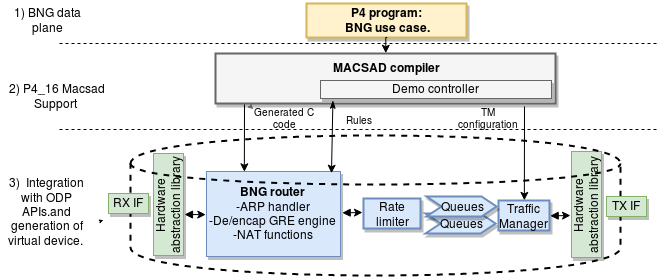
\includegraphics[width=0.7\linewidth] {figures/bng_arch_0.png}
	\caption{BNG software architecture.}
	\label{fig:bng_arch}
\end{figure*}


\begin{enumerate}
\item Create a P4 program in order to set the data plane functionalities of the BNG device (BNG data plane).   
\item Adds support the the current MACSAD implementation in order to compile the last version of P4 (P4\_16). 	
\item Integration of the BNG compiled and generated version by MACSAD with the ODP APIs, to add others features like Traffic management, Scheduling, and Rate limiter.

\end{enumerate}

Details of processes are explained in the next sections. It is important to highlight that the first process was completed, the second and third are currently in progress and the latter process is included as a scheduled task in Working Plan and Execution Schedule chapter.


\subsection{Creation of BNG data plane }
\label{ss:dataplane}
\begin{figure*}[ht]
	\centering
	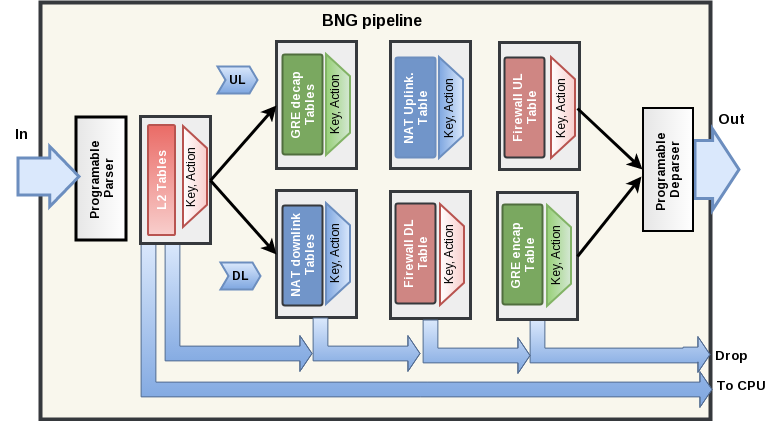
\includegraphics[width=0.7\linewidth] {figures/bng_pipe.png}
	\caption{BNG data plane.}
	\label{fig:bng_pipe}
\end{figure*}

To support the workload multiples lookup tables are supported either Upload link (UL) and Download Link (DL): a table to store MAC address, a table of CPE based on their IP address routing table, encap/decap GRE, both tables to block any port or IP using a Firewall for UL and DL, both table to Network Address translation (NAT) for UL and DL, the table to limiter the user rate either UL and DL. They are briefly described below.

\subsubsection{L2 mac table}
When the L2 packet is coming to the BNG switch, it uses MAC learning. Hence, when an ARP packet is received from the CPE, an entry is created (or updated) in a MAC address table swap the source and destination MAC address in the Ethernet header.\\
Ethernet is the protocol used in the Transport layer.  Therefore, the packet header fields are read and rewrite with the new fields in this table in order to forward the packet out by the appropriate port.

\subsubsection{Nat table}
Basic full-connect NAT for TCP traffic (over IPv4) do both main functions:
Translates IPv4 addresses and TCP port numbers of request packets originating from a client on a private network (iAddr: iPort) is mapped to an external address (eAddr: ePort), any packets from iAddr: iPort is sent through eAddr: ePort, the packets that his header fields matching in NAT table are processed in order to rewrite the new header and the packet is forwarded appropriately otherwise when a TCP packet is received on the external interface, for which there is no mapping, the packet is dropped.

\subsubsection{GRE tables}
The BNG will be able the forward based on the contents of a custom encapsulation header as well as perform normal IP forwarding if the encapsulation header does not exist in the packet.
Our BNG is enabled to create point-to-point tunnel mechanism in the intern network to encapsulate the packets with standard GRE packet header structure, as defined by RFC 2784 and RFC 2890 and save the user ID in order to establish the user session.\\
The BNG de-encapsulate the packets originated from CPE to an external address as well as the reverse process when the packet incoming from an external network.  The GRE table encap has the outer IP address header field in order add it as new IPv4 header and the GRE header fields in order to enable the new packet.

\subsubsection{IPV4 table}
The routing table stores the next hop based on the IP address. It’s based on the LPM (longest prefix match) implementation. Another table stores information related to the next hop (IP address, port index, etc.).
With IPv4 forwarding, the switch must perform the following actions for every packet: (i) update the source and destination MAC addresses, (ii) decrement the time-to-live (TTL) in the IP header, and (iii) forward the packet out the appropriate port.
Our BNG device will populate with static rules using a basic controller.  Each rule will map an IP address to the MAC address and output port for the next hop.

\subsubsection{Parser/Deparser}
Our parser will detect the different headers used in the BNG device. It extracts headers from the packet at the current offset into per-packet header instances and marks those instances valid, updating the Parsed Representation of the packet. The parser then indicates as valid byte the correct header and makes a state transition to the next header.
The de-parser reverses the process of parsing that emits headers in the proper order. Only headers which are valid are serialized, in our case, the output packet is serialized with the same protocols of the input parser block.

\subsubsection{Rate limiter}
Some research works [i.e \cite{Rodrigues},\cite{Popa},\cite{Ballani}]  based on end host-based rate enforcement for fair and guaranteed bandwidth allocation  in a  multi-tenant datacenter. 
A datacenter requires a large number of rate limiters, far of the capacity of commodity NICs (e.g., Intel’s 82599 10G NIC supports up to 128 rate limiters). Software rate limiters in host network stacks can scale, but this approach implies high CPU overheads hinder support for high-speed links \cite{Radhakrishnan_2014}
We implemented a basic Rate limiter in P4 code without slow down performance for every packet to inspect such as defined in RFC 2698 (A Two Rate Three Color Marker - IETF) standard; these describe traffic policing elements like a meter and a dropper.  The meter measures the traffic and determines whether or not it exceeds the rate limit, in case that it exceeds the limit the packets could be dropped.


\subsection{Macsad P4$_{16}$ support}
Macsad is in charge of converting our BNG P4 program into C code, specifically, it brings support to the version P4$_{14}$ (v1.0/v1.1). However, since may of 2017 has been launched the new version P4$_{16}$ (v1.0) that compared with the early version doing larges changes regarding syntax and semantics of the language.
The new P4$_{16}$ specification\footnote{https://p4lang.github.io/p4-spec/docs/P4-16-v1.0.0-spec.pdf} shows in figure \ref{fig:p4_evol} how this has been transformed from a complex language (more than 70 keywords) into a more compact language (less than 40 keywords) accompanied by a library of fundamental constructs that are needed for writing most of the P4 programs.

\begin{figure*}[ht]
	\centering
	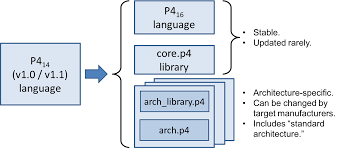
\includegraphics[width=0.7\linewidth] {figures/p4_evol.png}
	\caption{Evolution of the language between versions P4$_{14}$ (v 1.0 and 1.1) and P4$_{16}$.  
%  Source \cite{p4_evolu}}
    }
 	\label{fig:p4_evol}
 \end{figure*}

As we can see the section 
% \ref{sec:Macsad},
in the Frontend layer, MACSAD is using p4-hlir project which translates P4 programs into High-Level Intermediate Representation (HLIR) that creates a suitable P4 program representation (See figure \ref{fig:mac_arch}b), that can be consumed by multiple back-ends, in our case, MACSAD will be used this tool in “Transpiler module”, where is access the different P4 top-level objects using these Python ordered dictionary such as p4\_parser, p4\_tables, p4\_actions, p4\_headers and so on.\\
Therefore, our approach for MACSAD update to the new version is using HLIR16 project 
% \cite{hlir16}
that create a convenient Python representation from a JSON file compiled in P4C compiler from a .p4 source file. 


\subsection{Integration with OPD API's}

In order to apply some quality-of-services options for the ISP users, exist some mechanism for achieving these kinds of traffic-management goals in a shared network is through queuing and scheduling. This below features working together, deciding what packets get sent and when; thus scheduling is in charge of sending someone else’s packets right now or delaying packets that are arriving too fast.
In the following subsection, we will take a look at so-called Weighted fair queuing (WFQ) that provides a straightforward strategy for dividing bandwidth among multiple senders according to preset percentages.


\subsubsection{Weighted fair queuing (WFQ)} 

% \begin{figure}[ht]
% \centering
%   \subfigure[]
%   {
%     \raisebox{10mm}
%     {
%       \includegraphics[scale=0.5] 
%       {figures/wfq_diag.pdf}
%       \label{fig:wfq_diag}
%     }
%   }
%   \subfigure[]
%   {
%   	\includegraphics[scale=0.2]
%     {figures/tm_node.png}
%     \label{fig:tm_Node}
%   }
% \caption{(a)Weighted Fair Queuing priority.  Source (b) Traffic Manager Node.  Source  }
% \end{figure}


% \caption{(a)Weighted Fair Queuing priority.  Source \cite{anintro} (b) Traffic Manager Node.  Source \cite{opd_spec} }
% \end{figure}



This is a data packet scheduling algorithm based on both Fair Queueing (FQ) and the generalized processor sharing policy (GPS), where instead of giving each class an equal share, we assign each class a different percentage. For example, If all four input classes A,B,C,D are active, then each gets 25\% of the total bandwidth (see figure \ref{fig:wfq_diag}), just as for a flat four-input-class fair queuing structure. However, when only A, B and C are active, and D is idle.  A, B and C each get 33\%, hence it lets to allocate bandwidth according to administratively determined percentages.\\ 
ODP provides a suite of APIs that control traffic shaping and Quality of Service (QoS). Tx processing using Traffic manager and RX processing involves the use of Scheduler, both processes are described around in the next subsections.


\subsubsection{Scheduled RX Processing}
Scheduled RX processing is performed via the Scheduler and is requested when a PktIO is opened with an in\_mode of ODP\_PKTIN\_MODE\_SCHED.
In a basic use, it associates the PktIO input event queues created by odp\_pktin\_queue\_config() with the scheduler. The hash function could be employed to distribute input packets among multiple input queues and instead of these being plain queues they have scheduled queues and have associated scheduling attributes like the priority, scheduler group, and synchronization mode (parallel, atomic, ordered). 



% \subsubsection{Scheduled RX Processing}
% Scheduled RX processing is performed via the Scheduler and is requested when a PktIO is opened with an in\_mode of ODP\_PKTIN\_MODE\_SCHED.
% In a basic use, it associates the PktIO input event queues created by odp\_pktin\_queue\_config() with the scheduler. The hash function could be employed to distribute input packets among multiple input queues and instead of these being plain queues they have scheduled queues and have associated scheduling attributes like the priority, scheduler group, and synchronization mode (parallel, atomic, ordered). 
 \begin{figure}[ht]
 	\centering
 	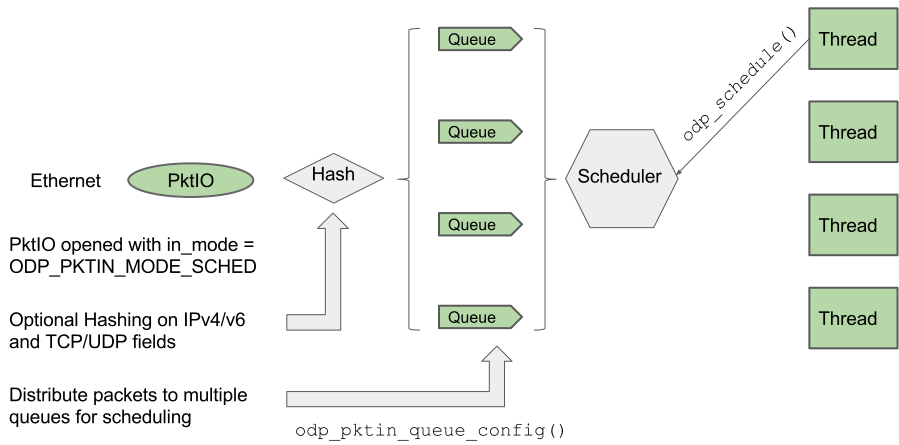
\includegraphics[width=0.55\linewidth] 
     {figures/pktin_sched_recv.png}
  	\caption{PktIO SCHED Mode Receive Processing.  Source} 
% \cite{opd_spec}}
 	\label{fig:pktin_sched}
 \end{figure}

Inbound packets are classified and put on queues associated with their target class of service which are themselves scheduled to threads (see figure \ref{fig:pktin_sched}). 

\subsubsection{Scheduled TX Processing}

Scheduled TX processing is performed via the ODP Traffic Manager and is requested when a PktIO is opened with an out\_mode of ODP\_PKTOUT\_MODE\_TM. 
The ODP Traffic Manager accepts packets from input queues and applies strict priority scheduling such as weighted fair queueing scheduling and bandwidth controls to decide which input packet should be chosen as the next output packet and when this output packet can be sent onwards.\\
Weighted Fair Queuing (WFQ) is used for priority assign from multiple input packets with the same priority. Each input can be assigned a weight in the range MIN\_WFQ\_WEIGHT to MAX\_WFQ\_WEIGHT (nominally 1..255) that affects the way the algorithm chooses the next packet. If all of the weights are equal AND all of the input packets are the same length then the algorithm is equivalent to a round-robin scheduling.\\

A TM system is composed of Tm\_nodes are "entity"/object. It lets interconnect, and interplay of a multi-level "tree" of tm\_nodes can allow the user to specify some very sophisticated behaviors. Each tm\_node can contain a set of WFQ scheduler (see figure \ref{fig:tm_Node}).  Each node contains a set of "fan-in" connections to preceding tm\_queues or tm\_nodes.
